\documentclass[a4paper,twoside]{bth}
% BTH THESIS TEMPLATE
%--------------------
% Template version 4.1 -- November 16, 2023
% Update also the Word template. Keep the version numbers in both formats in sync.
%--------------------
% Please change the data below appropriately to fit your thesis.
% The data will be used to generate text in various places on the
% thesis front and inner pages.
%--------------------

% DEGREE NAME. The degree name you are submitting your thesis for.
\newcommand{\thesisDegree}{Bachelor of Science in Software Engineering}

% DATE. The month year when your final report was submitted.
\newcommand{\thesisMonth}{May}
\newcommand{\thesisYear}{2024}

% FACULTY.
% Must be either Computing or Engineering.
\newcommand{\faculty}{Faculty of Computing}

% COURSE TIME. Course time in weeks.
% For a 15 credits course this should be 10 and
% for a 30 credits course, this should be 20 weeks.
% Note that the week figure is the same whether you work alone or in a pair.
\newcommand{\thesisWeeks}{Weeks}

% TITLE.
\newcommand{\thesisTitle}{Generative AI’s impact on user interfaces in data-intensive web applications: An exploratory analysis}

% SUBTITLE.
% If you do not have a subtitle, please delete the line below.
\newcommand{\thesisSubtitle}{Centered Subtitle in Font Times (Size 16 Bold)}

% AUTHORS.
% Please replace with your first name(s) and last name(s). There can be several of each.
\newcommand{\authorFirst}{Kasper Falk}
\newcommand{\authorFirstMail}{kafa21@student.bth.se}
% If there is no second author, please delete the texts in the last parentheses.
\newcommand{\authorSecond}{Joel Funk Persson}
\newcommand{\authorSecondMail}{jopl16@student.bth.se}

% University Advisor.
\newcommand{\super}{Eriks Klotins}
\newcommand{\superAffiliation}{Software Engineering}

% Company Advisor.
\newcommand{\superCompany}{Richard Houltz}
\newcommand{\superCompanyAffiliation}{Connectitude AB}
\newcommand{\superCompanyMail}{richard.houltz@connectitude.com}


% PACKAGES AND COMMANDS START
%----------------------------
% please do not delete or change anything before the END of this section
\usepackage[utf8]{inputenc}
\usepackage[T1]{fontenc}
\usepackage{graphicx}
\usepackage{amsmath}
\usepackage{mathenv}
\usepackage{amssymb}
\usepackage{amsthm}
\usepackage{textcomp}
\usepackage{longtable}
\usepackage{multirow}
\usepackage{booktabs}
\usepackage{caption}
\usepackage{pifont}
\usepackage{changepage}
\usepackage{listings}
\usepackage{nameref}
\usepackage{hyperref}
\usepackage{xspace}
\usepackage{xtab}
\usepackage{enumitem}
%\usepackage[sort&compress,numbers,square,comma]{natbib} % natbib interferes with the style; use \cite instead (see below)
\usepackage{cite} % works only with numeric citations; comment out when using author-year styles
\usepackage[color=blue!10,textsize=footnotesize,textwidth=25mm]{todonotes}
\DeclareGraphicsExtensions{.pdf}

\newtheorem{lem}{\textsc{Lemma}}[chapter]
\newtheorem{thm}{\textsc{Theorem}}[chapter]
\newtheorem{prop}{\textsc{Proposition}}[chapter]
\newtheorem{post}{Postulate}[chapter]
\newtheorem{corr}{\textsc{Corollary}}[chapter]
\newtheorem{defs}{\textsc{Definition}}[chapter]
\newtheorem{cons}{\textsc{Constraint}}[chapter]
\newtheorem{ex}{\textbf{Example}}[chapter]
\newtheorem{qu}{\textbf{Question}}[chapter]
% -------------------------
% PACKAGES AND COMMANDS END


% DOCUMENT BEGINS HERE
\begin{document}

\pagestyle{plain}
\pagenumbering{roman}

% THESIS FRONT PAGE (please do not change)
% ----------------------------------------
{\pagestyle{empty}
\changepage{3cm}{1cm}{-0.5cm}{-0.5cm}{}{-1.5cm}{}{}{}
\noindent
\begin{tabular}{@{}p{0.75\textwidth} p{0.25\textwidth}}
\thesisDegree & \hfill\multirow{3}{*}{\bthcsnotextlogo{3cm}} \\
\thesisMonth \ \thesisYear & \\
\end{tabular}

%\begin{center}
\center
\vspace {7.5cm}
{\Huge\textbf{\thesisTitle}}

\vspace {0.5cm}
{\Large\textbf{\thesisSubtitle}}

\vspace{2cm}
{\Large\textbf{\authorFirst}}

\vspace{0.3cm}
{\Large\textbf{\authorSecond}}

\vspace*{\fill}

\noindent\makebox[\linewidth]{\rule{\textwidth}{1pt}} 
Faculty of \faculty, Blekinge Institute of Technology, 371 79 Karlskrona, Sweden
%\end{center}

\clearpage
} % Back to \pagestyle{plain}
% ----------------------------------------


% THESIS INNER PAGE (please do not change)
% ----------------------------------------
{\pagestyle{empty}
\changepage{3cm}{1cm}{-0.5cm}{-0.5cm}{}{-1.5cm}{}{}{}

{\small
\noindent
This thesis is submitted to the Faculty of \faculty\ at Blekinge Institute
of Technology in partial fulfillment of the requirements for the degree of
\thesisDegree. The thesis is equivalent to \thesisWeeks\ weeks of full-time studies.

\vspace{1cm}

\noindent
The authors declare that they are the sole authors of this thesis and that they have
not used any sources other than those listed in the bibliography and identified as references.
They further declare that they have not submitted this thesis at any other institution to
obtain a degree.
}

\vspace{10cm}

\noindent
\textbf{Contact Information:} \\
Author(s): \\
\authorFirst \\
E-mail: \authorFirstMail \\
\\
\authorSecond \\
E-mail: \authorSecondMail

\vspace{2cm}

\noindent
University advisor: \\
\super \\
Department of \superAffiliation

\vspace{1cm}

\noindent
Compnay advisor: \\
\superCompany \\
\superCompanyAffiliation \\
E-mail: \superCompanyMail

\vspace*{\fill}

\noindent
\begin{tabular}{@{}p{0.5\textwidth} l c l}
Faculty of \faculty              & Internet & : & www.bth.se \\
Blekinge Institute of Technology & Phone    & : & +46 455 38 50 00 \\
SE--371 79 Karlskrona, Sweden    & Fax      & : & +46 455 38 50 57 \\
\end{tabular}
\clearpage
} % Back to \pagestyle{plain}
% ----------------------------------------

\setcounter{page}{1}

%%%%%%%%%%%%%%%%%%%%%%%%
% TEXTS START HERE
%%%%%%%%%%%%%%%%%%%%%%%%

% ABSTRACT IN ENGLISH
% -------------------
\abstract
Abstract Text Here
\clearpage
% -------------------
% ACKNOWLEDGEMENTS
% -------------------
\acknowledgments
\noindent
Add acknowledgements here.

\clearpage
% -------------------


% TABLE OF CONTENTS PAGES (generated by LaTeX using the command(s) below)
\setcounter{secnumdepth}{3} % only include sections down to level 3
\tableofcontents
% You should uncomment the commands you need.
%\listoffigures             % in case you have them
%\listoftables              % in case you have them
%\listofalgorithms          % in case you have them

\cleardoublepage
\pagestyle{headings}
\pagenumbering{arabic}

%%%%%%%%%%%%%%%%%%%%%%%%
% Introduction | Chapter 1
%%%%%%%%%%%%%%%%%%%%%%%%
%%%%%%%%%%%%%%%%%%%%%%%%
% Introduction | Chapter 1
%%%%%%%%%%%%%%%%%%%%%%%%
\chapter{Introduction}
\label{chp:introduction}  % labels are used for cross references

\section{Background}
Today, technological developments are advancing at an increasingly rapid pace, opening up new opportunities and challenges in software engineering. A particularly interesting and critical research area that is emerging is generative AI (artificial intelligence). This technology has caught the interest of many companies who see the potential of integrating generative AI into their web applications. Through this, user interfaces can become more intuitive and accessible, which can significantly improve the user experience.

One example of a company exploring this technology is Connectitude AB. They are particularly interested in how generative AI can be applied in their data-intensive web applications to simplify the analysis and interpretation of large amounts of data for the users. In our bachelor thesis, in collaboration with Connectitude AB, we will explore how generative AI can influence the user experience in web applications that require extensive data processing. Our goal is to identify both the positive and negative aspects of employing generative AI in settings that demand significant data handling, particularly those relating to certain aspects of user experience, such as usability(learnability, understandability) and efficiency.

\section{Motivation and Value}
With this research we want to inform the public and businesses about the value of generative AI in data-intensive web applications. Also by highlighting the limitations and challenges of using generative AI in environments that require extensive data processing. We believe it can lead to a better understanding of the current capabilities and areas for improvement, especially in usability concerning learnability and understandability.

Data presented in a data-intensive web application can sometimes be very difficult to interpret for a user, but with the help of generative AI, data can be made more understandable and user-friendly. This can help increase usability and value compared to previous methods. By integrating generative AI into a data-intensive web application, we believe it can offer users greater learning ability and reduce the time spent pondering what to do next when dealing with a data-intensive application, especially for those who are not so technical.

The article "Generative AI at work"  addresses whether using generative AI increases productivity for employees but also improvements in problem solving for those who are new workers or less technical. Providing generative AI can simplify information access for individuals with different levels of knowledge and make it more user-friendly by typing to a chatbot instead of looking around the application and trying to find what you are looking for. This approach can also reduce the steep learning curve traditionally associated with these applications.

\section{Scope}
In our bachelor thesis in software engineering, we want to explore the use of generative artificial intelligence in user experience and data management in web applications. By exploring generative AI in a user interface of a data-intensive web application, we want to understand and analyze its impact on the user experience.

Our study focuses on the impact of generative AI on usability in learning ability and understandability. We also aim to explore how generative AI is perceived by different skilled users. A further focus area is to assess the quality and relevance of the information generated by generative AI. We want to explore how well generative AI can analyze and adapt data to provide more insightful and relevant information.

Through this research, we hope to contribute insights into how generative AI can be used to improve user experience in data-intensive applications, and how these techniques can be adapted to meet the needs of a broad user base.

Our study aims to put generative AI in a broader societal context, to understand its potential and limitations in terms of user experience in web applications.

\section{outline}
Outline text here


%%%%%%%%%%%%%%%%%%%%%%%%
% Related work | Chapter 2
%%%%%%%%%%%%%%%%%%%%%%%%
%%%%%%%%%%%%%%%%%%%%%%%%
% Related work | Chapter 2
%%%%%%%%%%%%%%%%%%%%%%%%
\chapter{Related Work}
\label{chp:relatedwork}
Related work text here


%%%%%%%%%%%%%%%%%%%%%%%%
% Method | Chapter 3
%%%%%%%%%%%%%%%%%%%%%%%%
%%%%%%%%%%%%%%%%%%%%%%%%
% Method | Chapter 3
%%%%%%%%%%%%%%%%%%%%%%%%
\chapter{Method}
\label{chp:method}

\section{Research questions}
Main question
\begin{itemize}
    \item RQ1. Can the use of generative AI help improve the user experience in a data-intensive web application compared to traditional user interface methods?
\end{itemize}

Sub questions
\begin{itemize}
    \item RQ1.1. To what extent can generative AI improve the usability of a UI?

    With this research question we aim to explore the understandability of the UI. We will measure understandability by accounting for pondering time, and users asking for clarifications.

    \item RQ1.2. What are the key challenges for non-technical users using generative AI for data visualization in web applications?

    \item RQ1.3: Can generative AI help to improve perceived efficiency and task completion when working with a data-intensive web application?

    With this research question, we aim to explore efficiency in terms of tasks completed per time but also the perceived efficiency. We will measure efficiency by accounting for time spent per task and total tasks completed. The perceived efficiency will be measured through qualitative data collected in the exit interview.
    
\end{itemize}

\section{Literature review}
Search Strings used on Scopus
In order to locate the most relevant studies for our research on the impact of generative AI on user interfaces in data-intensive web applications, we have designed a search strategy to be employed within Scopus. The following search strings were used:

\begin{itemize}
    \item TITLE-ABS-KEY ( ( "generative AI" OR "generative artificial intelligence" ) AND ( "user interface" OR accessibility OR usability ) ) AND ( LIMIT-TO ( PUBSTAGE , "final" ) ) AND ( LIMIT-TO ( SUBJAREA , "COMP" ) OR LIMIT-TO ( SUBJAREA , "ENGI" ) OR LIMIT-TO ( SUBJAREA , "SOCI" ) OR LIMIT-TO ( SUBJAREA , "DECI" ) OR LIMIT-TO ( SUBJAREA , "BUSI" ) OR LIMIT-TO ( SUBJAREA , "ENVI" ) ) AND ( LIMIT-TO ( LANGUAGE , "English" ) )

    \item TITLE-ABS-KEY ( ( "data-intensive" OR "data intensive" ) AND "Web application" AND ( "user interface" OR accessibility OR usability ) ) AND ( LIMIT-TO ( PUBSTAGE , "final" ) ) AND ( LIMIT-TO ( SUBJAREA , "COMP" ) OR LIMIT-TO ( SUBJAREA , "ENGI" ) OR LIMIT-TO ( SUBJAREA , "SOCI" ) OR LIMIT-TO ( SUBJAREA , "DECI" ) OR LIMIT-TO ( SUBJAREA , "BUSI" ) OR LIMIT-TO ( SUBJAREA , "ENVI" ) ) AND ( LIMIT-TO ( LANGUAGE , "English" ) )
\end{itemize}

\section{Data Collection}
We are using a mix of different methods to collect data. These include a demographic survey, a “thing” and an exit interview.

To collect data for our “thing” we are using a mix of different methods. We are gathering quantitative data through our demographic survey, where we get information about our participants and the experience.

To collect data “that is relevant to the whole thing” we are going to perform an “experiment/observation thing”, where our participants perform data analysis tasks on a web application. Half of the participants will use a traditional application and the other half will also have access to a generative AI(that has access to the data the application has).

During the “thing”, the participants are prompted to verbalize their thoughts(thinking aloud), this will help us get as much data as possible from the few participants we are able to perform the experiment with. After the “thing” we will gather more qualitative data from an exit interview.

\subsection{Demographic Survey(Google Forms):}
To be performed before the session. With the intent of gathering information about our participants to understand their background and experience with technology, their occupation aswell as age. We will also inform the participants what the experiment will entail, including information about how the experiment will work, that they will be recorded and how the collected data will be used.

\begin{itemize}
    \item Inform and Get Consent: We are going to clearly explain the purpose of the study, what participation involves, risks, benefits, and confidentiality of responses. We will also ensure that our participants understand their rights, including withdrawal at any time without penalty. Obtain written or digital consent.
\end{itemize}
\begin{itemize}
    \item Age: To understand the age distribution of our participants.
    \item Experience: Gauge the overall experience level with technology, specifically web applications and AI tools.
    \item Experience in What: Understand the domains of their experience, e.g., software development, design, data analysis, etc.
    \item Occupation Information: Collect data on their current job roles to understand their professional background.
    \item Inform About the Observation: Detail what the observation will entail, including the tasks to be performed, the use of recording equipment (if any), and how the collected data will be used.
\end{itemize}

\subsection{Session preparation (On-site)}
To be done before each session/participant. We will setup the application, with or without the AI component depending on the treatment for that participant. Have the necessary programs running and making sure it looks the same for each participant. Tasks will be prepared and printed out so the participant can read at their own discretion if necessary.

<----- Picture here ------>

\begin{itemize}
    \item Setup Experiment Environment Beforehand: Ensure the application and all necessary tools are functioning and running correctly. Also that everything is set up exactly the same for each participant.
    \item Load Application: Have the application ready on the device that will be used for the observation.
    \item Load Generative AI Part: Ensure that the generative AI component of the application is set up and ready to interact with.
    \item Load Task Instructions: Prepare clear and concise instructions for the tasks participants will perform.
\end{itemize}

\subsection{Session steps (On-site) ~30 min}
To be performed with each participant. Th
\begin{itemize}
    \item Start Recording: Begin recording the session, ensuring to capture both the participant's interactions with the application and their verbal feedback.
    \item Explain the Application and Its Functionality: Provide a brief overview of the application, focusing on its purpose and key features.
    \item Explain Task Performance: We will describe how participants should perform the tasks by including any specific requirements/rules and guidelines. Explain that they will be given one task at a time, and upon completion or aborting of a task, the next one will be given to them. The tasks will start off short and easy and then increase in difficulty. Estimated time per task will vary, ranging from ~1-2 minutes to ~5-10.
    \item Instruct Them to Speak Out Loud: We will encourage participants to verbalize their thoughts, feelings, and frustrations as they interact with the application.
    \item Task Performance: Allow participants to start performing the tasks, observing and taking notes on their interactions and feedback. When a participant is done with a task, the next one will be given to them.
    \item Prompt to Speak if Necessary: If participants become silent, we will remind them to share their thoughts.
    \item Measure Task Completion Time: Record the time it takes for participants to complete each task.
    \item End of Observation: Conclude the task performance phase and stop the recording.
\end{itemize}

\subsection{Exit Interview (Semi-structured, On-site) ~15 min:}
\begin{itemize}
    \item Productivity Feelings: Ask participants about their perceived productivity while using the application. There we are focusing on their feelings rather than trying to quantify actual productivity.
    \item Ease of Use: Ask about the application's usability, how easy it was to accomplish basic tasks, how many mistakes (errors) were made, and whether participants found it intuitive and straightforward to navigate.
    \item Understanding and Starting Points: Assess whether participants knew how to start interacting with the application and the AI components, and if the UI effectively guided them in understanding what to do next.
    \item Satisfaction: Gather feedback on how satisfying participants found the application to use, including any particular features or interactions that stood out.
    \item General feedback: Ask the participant for any additional remarks, comments, or preferences about their experience that could be useful for evaluating the UI.
\end{itemize}

\subsection{Session conclusion}

%%%%%%%%%%%%%%%%%%%%%%%%
% Results and Analysis | Chapter 4
%%%%%%%%%%%%%%%%%%%%%%%%
%%%%%%%%%%%%%%%%%%%%%%%%
% Results and Analysis | Chapter 4
%%%%%%%%%%%%%%%%%%%%%%%%
\chapter{Results and Analysis}
\label{chp:results}

\section{RQ1.1. To what extent can generative AI improve the usability of a UI?}
\subsection{Visualisation of the data}
\subsection{Answer to the research question}
Snacka lite om interjuverna detta med att AI hjälper med Uiet:
Ta upp om att man kan kolla om man är på rätt spår (får smama svar som AI / man kollar på samma data)

\section{RQ1.2. What are the key challenges for users using generative AI for data visualization in web applications?}
\subsection{Visualisation of the data}
\subsection{Answer to the research question}

\section{RQ1.3: Can generative AI help to improve perceived efficiency and task completion when working with a data-intensive web application?}
\subsection{Visualisation of the data}
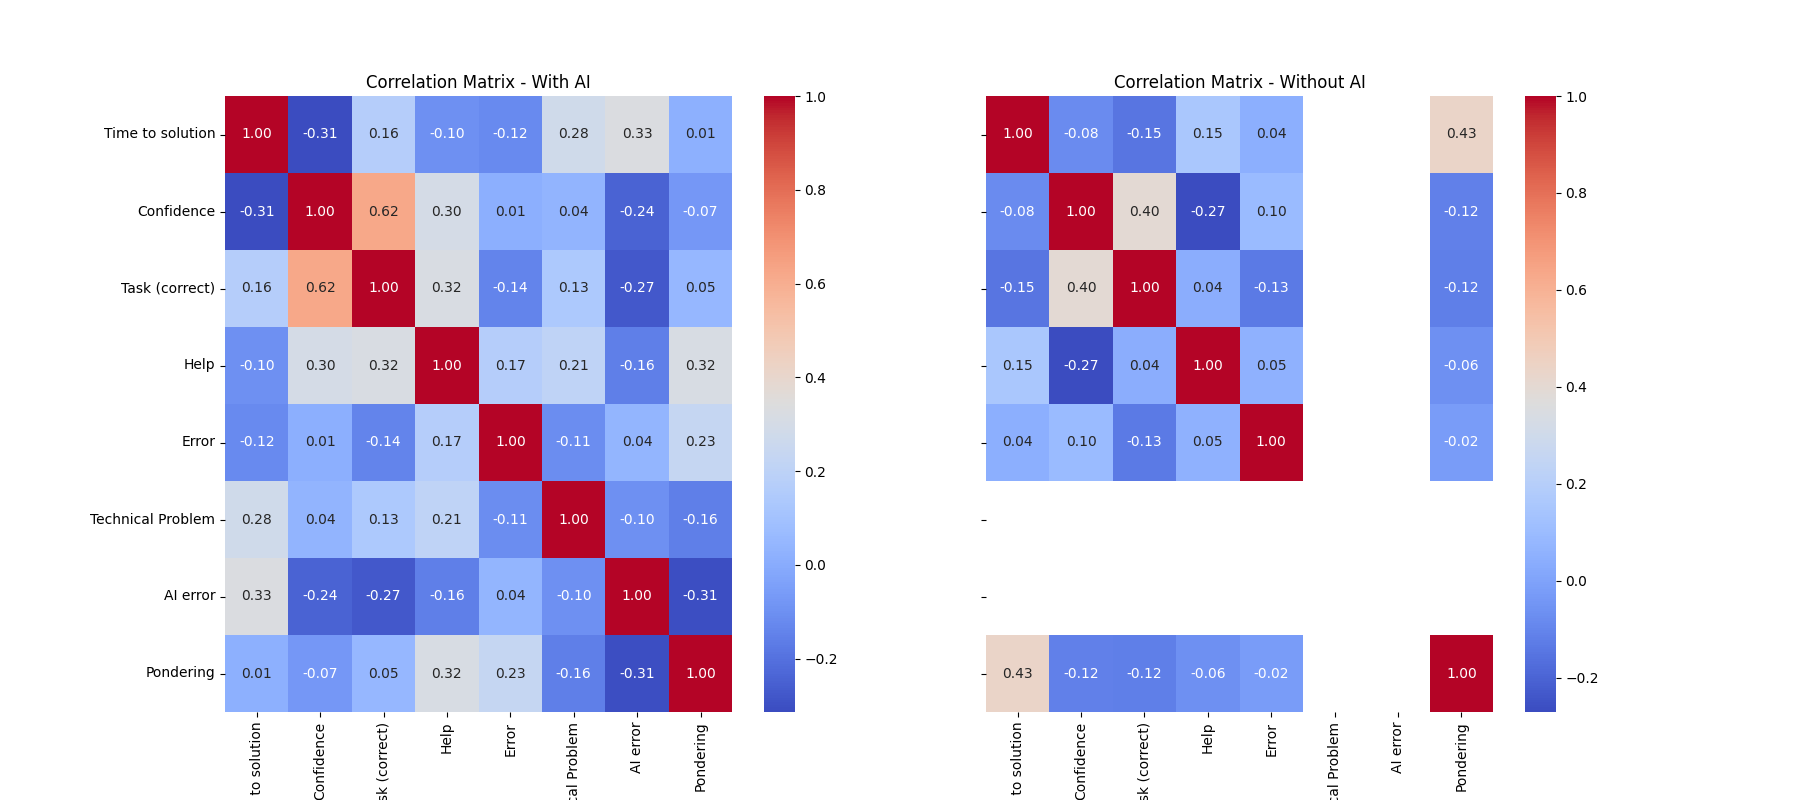
\includegraphics[width=\textwidth]{Images/correlation_matrix_split_treatment.png}
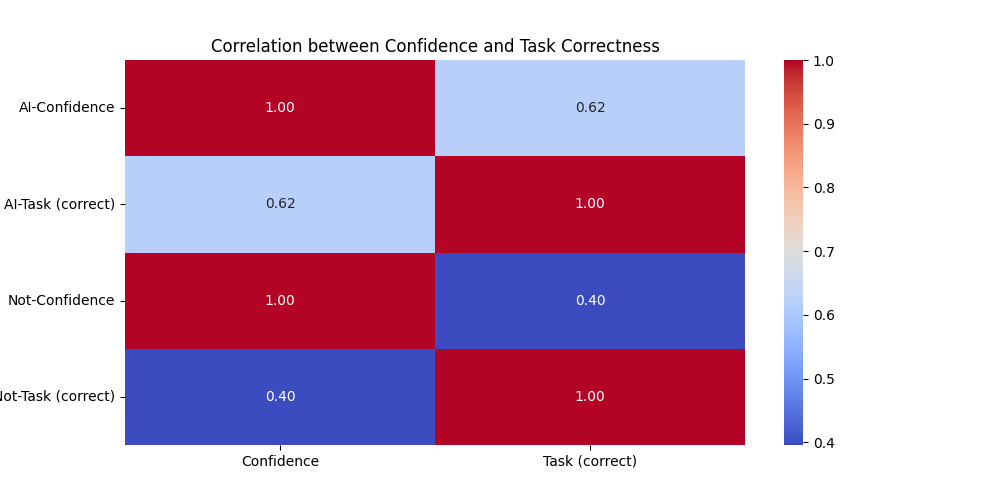
\includegraphics[width=\textwidth]{Images/confidence_correlation_heatmap.png}
 - Confidence in task results seem to correlate more with actual results when using AI.
 - Generally slower results produced, atleast in a small scale like this.
 - Accuracy in answers are also lower when using AI.
 - The slower and less accurate results probably has more to do with the implementation of the AI itself rather than the usage AI could possibly have in data intensive applications.
\subsection{Answer to the research question}

\section{RQ1. Can the use of generative AI help improve the user experience in a data-intensive web application compared to traditional user interface methods?}
\subsection{Visualisation of the data}
\subsection{Answer to the research question}


%%%%%%%%%%%%%%%%%%%%%%%%
% Discussion | Chapter 5
%%%%%%%%%%%%%%%%%%%%%%%%
%%%%%%%%%%%%%%%%%%%%%%%%
% Discussion | Chapter 5
%%%%%%%%%%%%%%%%%%%%%%%%
\chapter{Discussion}
\label{chp:discussion}
\section{On the content}
In many theses, the discussion is the most important section. Make sure that you allocate enough time and space for a good discussion. This is your opportunity to show that you have understood the significance of your findings and that you are capable of applying theory in an independent manner.

The discussion will consist of argumentation. In other words, you investigate a phenomenon from several different perspectives. To discuss means to consider different interpretations of your findings. Here are a few examples of formulations that signal argumentation:

\begin{itemize}
    \item On the one hand \dots and on the other \dots 
    \item However \dots
    \item \dots it could also be argued that \dots
    \item Another possible explanation may be \dots
\end{itemize}


\section{Things to keep in mind when writing your discussion}
\begin{enumerate}
    \item Try to structure your discussions from the ``specific'' to the ``general'': expand and transition from the narrow confines of your study (based on your results and analyses) to the general framework of your discipline.
    \item Make a consistent effort to stick with the same general tone of the introduction. This means using the same key terms, the same tense, and the same point of view as used in your introduction.
    \item Start by re-stating your research questions and/or hypotheses. Then declare the answers to them -- make sure to support these answers with a clear line of evidence that can be traced to your analysis and/or your data.
    \item Continue by explaining how your results relate to the expectations of your study and to the literature. Clearly explain why the results are trustworthy (or not if there are doubts about the reliability or validity of the data collection and/or analysis) and how they relate (supporting or contradicting) with previously published knowledge about the subject. If your thesis closes a research gap you or someone else has identified and described, state that explicitly. Make sure to use relevant citations.
    \item Make sure to give the proper attention to all the results relating to your research questions, this is regardless of whether or not the findings were statistically significant.
    \item Don't forget to tell your audience about the patterns, principles, and key relationships shown by each of your major findings and then put them into perspective. The sequencing of this information is important: 1) state the answer, 2) show the relevant results and 3) cite the work of credible sources. When necessary, point the audience to figures and/or graphs to ``enhance'' your argument.
    \item Make sure to justify your answers. Try to do so in two ways: by explaining the validity of your answer and by showing the potential shortcomings of others' answers. You will make your point of view more convincing if you provide both sides to the argument.
    \item Also make sure to identify conflicting data in your work. Make a good point of discussing and evaluating any conflicting explanations of your results. This is an effective way to win over your audience and make them sympathetic to any true knowledge your study might have to offer.
    \item Make sure to include a discussion of any unexpected findings. When doing this, begin with a paragraph about the finding and then describe it. Also, identify potential limitations and weaknesses inherent in your study. Then comment on the importance of these limitations to the interpretation of your findings and how they may impact their validity. Do not use an apologetic tone in this section. Every study has limitations. Showing your awareness regarding the limitations increases the trustworthiness of your reasoning.
    \item Conduct a brief summary of the principal implications of your findings for research and practice in the area (do this regardless of any statistical significance). You might also want to provide recommendations for potential research in the future related to your implications. A brief summary of these recommendations will typically be included in Chapter~\ref{chp:conclusions} (\emph{\nameref{chp:conclusions})}.
    \item You should also think about the potential wider consequences of your results. Do they have an impact on society? What are the possible ethical consequences of your findings? Does your work have an impact on sustainability (in whatever dimension)?
%    \item Show how the results of your study and their conclusions are significant and how they impact our understanding of the problem(s) that your thesis examines. This will make the contribution of your thesis more explicit.
    \item On a final note, discuss everything that is relevant \emph{but be brief, specific, and to the point}.
\end{enumerate}





% All references are in a separate file: thesis-refs.bib
\bibliography{thesis-refs}
\bibliographystyle{IEEEtranS}


\appendix
\chapter{Supplemental Information}


% DO NOT CHANGE BELOW
% This part makes sure that the last page is even with BTH-logo.
% -------------------
\cleardoublepage
\thispagestyle{empty}
\vspace*{\fill}
\clearpage{\thispagestyle{empty}}
\changepage{3cm}{1cm}{-0.5cm}{-0.5cm}{}{-1.5cm}{}{}{}
\vspace*{\fill}
\center

{\bthcsnotextlogo{3cm}}
\\
\noindent\makebox[\linewidth]{\rule{\textwidth}{1pt}} 
Faculty of \faculty, Blekinge Institute of Technology, 371 79 Karlskrona, Sweden
% -------------------

\end{document}
